\begin{figure}[!ht]
\begin{center}
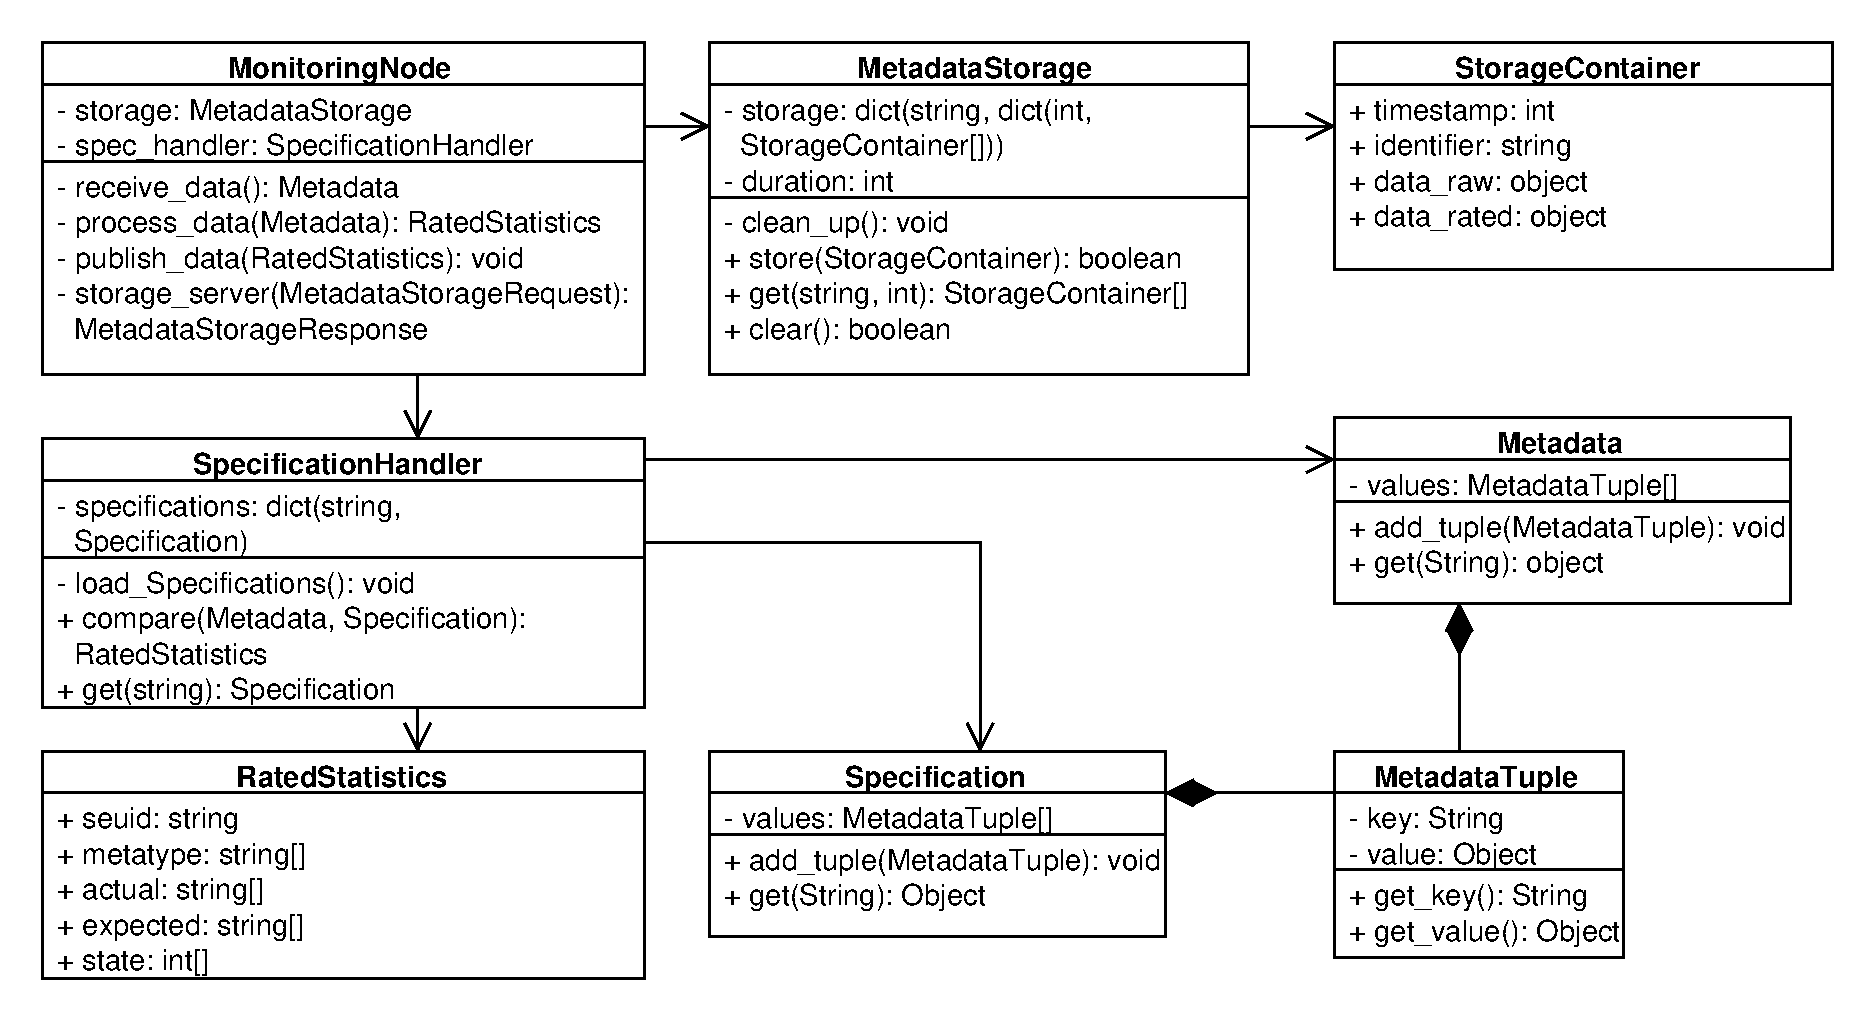
\includegraphics[width=1.0\linewidth]{./diagram_pictures/processing.pdf}
\caption{The UML diagram of the processing package}
\end{center}
\end{figure}

\mbox{}

\newpage

\subsection{MonitoringNode}
\begin{figure}[htbp]
	\begin{minipage}[t]{7cm}
		\vspace{0pt}
		\centering
		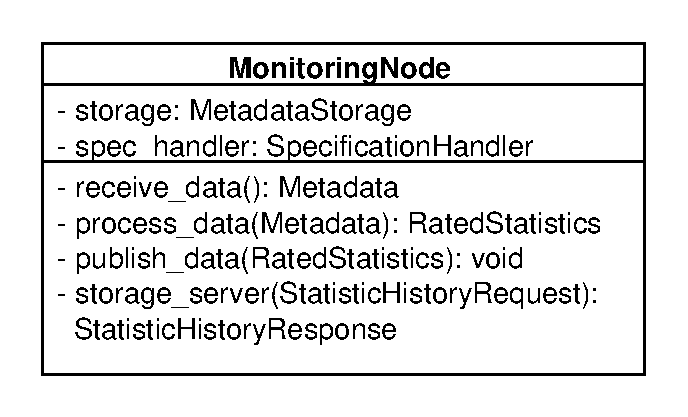
\includegraphics[scale=0.6]{./diagram_pictures/MonitoringNode.pdf}
		\caption{The MonitoringNode}
	\end{minipage}
	\hfill
	\begin{minipage}[t]{8cm}
		\vspace{10pt}
		Main Class wrapping the processing functionality.
	\end{minipage}
\end{figure}

\subsubsection{Attributes}
\begin{itemize}
	\item \textbf{private MetadataStorage storage}
	\item \textbf{private SpecificationHandler specHandler}
\end{itemize}
\subsubsection{Methods}
\begin{itemize}
	\item \textbf{private void receive\_data()}\\
	Receives data incoming from the Subscriber and converts them to Metadata objects.
	\item \textbf{private RatedStatistics process\_data(Metadata)}\\
	Returns the specHandler's compare result
	\item \textbf{private void publish\_data(RatedStatistics)}\\
	Publishes results of the comparison as rated Metadata
	\item \textbf{private StatisticHistoryResponse storage\_server(StatisticHistoryRequest)}\\
	Listens for the GUI Model service calls and returns requested metadata from the storage
\end{itemize}

\newpage
\subsection{MetadataStorage}
\begin{figure}[htbp]
	\begin{minipage}[t]{7cm}
		\vspace{0pt}
		\centering
		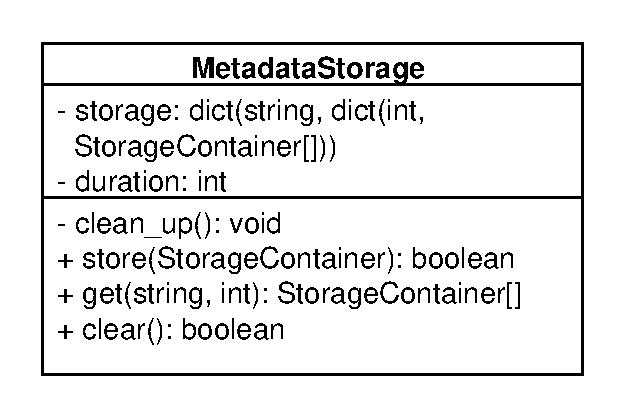
\includegraphics[scale=0.6]{./diagram_pictures/MetadataStorage.pdf}
		\caption{The MetadataStorage}
	\end{minipage}
	\hfill
	\begin{minipage}[t]{8cm}
		\vspace{10pt}
		Saves received metadata packages for a given period of time and can provide them on request.
	\end{minipage}
\end{figure}

\subsubsection{Attributes}
\begin{itemize}
	\item \textbf{private dict(string, dict(int, StorageContainer[])) storage}\\
	Datastructure to store Packages by key and timestamp.
	\item \textbf{private int duration}\\
	The duration in seconds for data to be stored.
\end{itemize}
\subsubsection{Methods}
\begin{itemize}
	\item \textbf{private void clean\_up()}\\
	Deletes Metadata exceeding the duration to store
	\item \textbf{public boolean store(StorageContainer)}\\
	Stores a given Metadata
	\item \textbf{public StorageContainer[] get(string, int)}\\
	Returns all Metadata packages for the given connection/host of the given amount of time.
	\item \textbf{public boolean clear()}\\
	Clears the whole storage
\end{itemize}

\newpage
\subsection{StorageContainer}
\begin{figure}[htbp]
	\begin{minipage}[t]{7cm}
		\vspace{0pt}
		\centering
		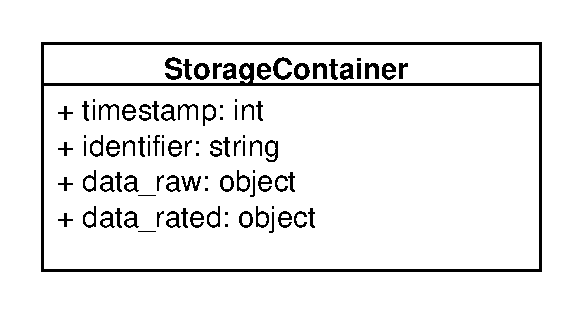
\includegraphics[scale=0.6]{./diagram_pictures/StorageContainer.pdf}
		\caption{The StorageContainer}
	\end{minipage}
	\hfill
	\begin{minipage}[t]{8cm}
		\vspace{10pt}
		Wraps Metadata in raw and rated form with an identifier and a timestamp. Object to be returned on request by the GUI model.
	\end{minipage}
\end{figure}

\subsubsection{Attributes}
\begin{itemize}
	\item \textbf{public int timestamp}\\
	Time when the data came from the subscriber.
	\item \textbf{public string identifier}\\
	Host/Node/Connection identifier
	\item \textbf{public object data\_raw}\\
	The data as it reaches the subscriber from nodes and hosts.
	\item \textbf{public object data\_rated}\\
	The data like it would be published after being rated.
\end{itemize}


\subsection{Metadata}
\begin{figure}[htbp]
	\begin{minipage}[t]{7cm}
		\vspace{0pt}
		\centering
		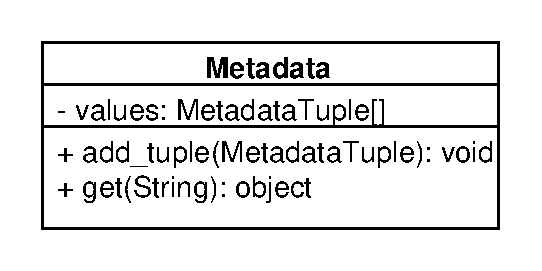
\includegraphics[scale=0.6]{./diagram_pictures/Metadata.pdf}
		\caption{The Metadata}
	\end{minipage}
	\hfill
	\begin{minipage}[t]{8cm}
		\vspace{10pt}
		Wraps metadata of exactly one host or node, a topic or a node-topic-combination.
	\end{minipage}
\end{figure}

\subsubsection{Attributes}
\begin{itemize}
	\item \textbf{private MetadataTuple[] values}\\
	Collection of Metadata regarding multiple meassurements.
\end{itemize}
\subsubsection{Methods}
\begin{itemize}
	\item \textbf{public void add\_tuple(MetadataTuple)}\\
	Add a MetadataTuple of information to the bundle.
	\item \textbf{public object get(String)}\\
	Returns the value of the MetadataTuple with the given key. False, if the key does not exist.
\end{itemize}


\subsection{Specification}
\begin{figure}[htbp]
	\begin{minipage}[t]{7cm}
		\vspace{0pt}
		\centering
		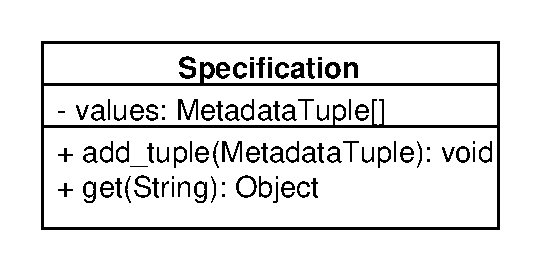
\includegraphics[scale=0.6]{./diagram_pictures/Specification.pdf}
		\caption{The Specification}
	\end{minipage}
	\hfill
	\begin{minipage}[t]{8cm}
		\vspace{10pt}
		An object loaded from the specification configurations and basis for comparison of Metadata with desired values.
	\end{minipage}
\end{figure}

\subsubsection{Attributes}
\begin{itemize}
	\item \textbf{private MetadataTuple[] values}\\
	Collection of MetadataTuple objects providing limits for multiple fields.
\end{itemize}
\subsubsection{Methods}
\begin{itemize}
	\item \textbf{public void add\_tuple(MetadataTuple)}\\
	Adds a MetadataTuple to the bundle
	\item \textbf{public Object get(String)}\\
	Returns the value of the MetadataTuple with the given key. The returned value would be a list containing limit values for the most measured fields. False, if the key does not exist.
\end{itemize}

\newpage
\subsection{SpecificationHandler}
\begin{figure}[htbp]
	\begin{minipage}[t]{7cm}
		\vspace{0pt}
		\centering
		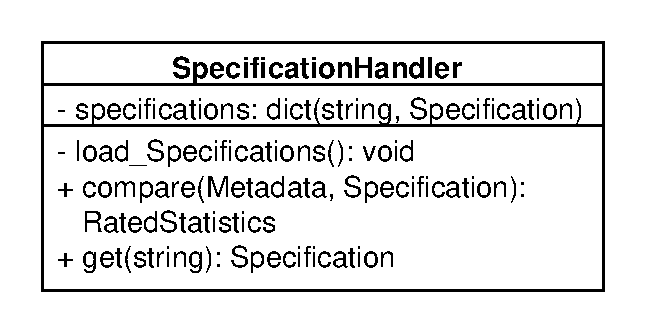
\includegraphics[scale=0.6]{./diagram_pictures/SpecificationHandler.pdf}
		\caption{The SpecificationHandler}
	\end{minipage}
	\hfill
	\begin{minipage}[t]{8cm}
		\vspace{10pt}
		Loads the specifications from the parameter server and compares them to the actual metadata.
	\end{minipage}
\end{figure}

\subsubsection{Attributes}
\begin{itemize}
	\item \textbf{private dict(string, Specification) specifications}\\
	Datastructure to keep all loaded Specification objects
\end{itemize}
\subsubsection{Methods}
\begin{itemize}
	\item \textbf{private void load\_specifications()}\\
	Loads the specifications from configuration files into Specification objects and stores them
	\item \textbf{public RatedStatistics compare(Metadata, Specification)}\\
	Compares a given Metadata object with a given Specification object regarding all available fields. Returns a RatedStatistics object wrapping potential divergences.
	\item \textbf{public Specification get(string)}\\
	Returns the specification for a given identifier
\end{itemize}


\subsection{RatedStatistics}
\begin{figure}[htbp]
	\begin{minipage}[t]{7cm}
		\vspace{0pt}
		\centering
		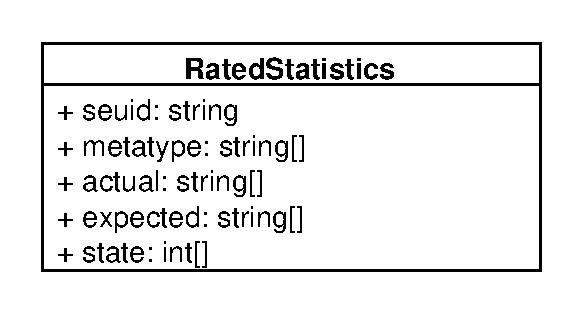
\includegraphics[scale=0.6]{./diagram_pictures/RatedStatistics.pdf}
		\caption{The RatedStatistics}
	\end{minipage}
	\hfill
	\begin{minipage}[t]{8cm}
		\vspace{10pt}
		Wraps the result of the comparison between the actual metadata and the specificaton.
	\end{minipage}
\end{figure}

\subsubsection{Attributes}
\begin{itemize}
	\item \textbf{public string seuid}\\
	Identifies the node/host/connection
	\item \textbf{public string[] metatype}\\
	The metadata that was out of bounds
	\item \textbf{public string[] actual}\\
	The actual values
	\item \textbf{public string[] expected}\\
	The expected values
	\item \textbf{public int[] state}\\
	State of the metadata from the node/host/connection : state: { 0 = high ; 1 = low ; 2 = unknown}
\end{itemize}


\subsection{MetadataTuple}
\begin{figure}[htbp]
	\begin{minipage}[t]{7cm}
		\vspace{0pt}
		\centering
		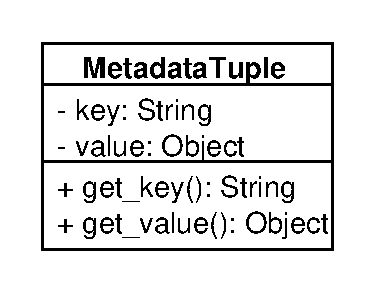
\includegraphics[scale=0.6]{./diagram_pictures/MetadataTuple.pdf}
		\caption{The MetadataTuple}
	\end{minipage}
	\hfill
	\begin{minipage}[t]{8cm}
		\vspace{10pt}
		Stores any kind of value for a certain key. Specifications storing values indicating limits, Metadata storing absolute actual values.
	\end{minipage}
\end{figure}

\subsubsection{Attributes}
\begin{itemize}
	\item \textbf{private String key}
	\item \textbf{private Object value}
\end{itemize}
\subsubsection{Methods}
\begin{itemize}
	\item \textbf{public String get\_key()}
	\item \textbf{public Object get\_value()}
\end{itemize}